\chapter{Einleitung}
\label{kap:einleitung}

\section{Aufgabenstellung}

Mobile Bauzaunfelder werden auf Baustellen und in Mietparks liegend gestapelt.
Für Inventur, Rückgabekontrolle und Abrechnung muss die Anzahl der Felder eines
Stapels bekannt sein. Gezählt wird bislang von Hand -- bei 50 bis 200 Feldern pro
Stapel ist das langsam und fehleranfällig, weil die Felder eng aufeinanderliegen
und sich in der Aufsicht kaum voneinander abgrenzen.

Die Aufnahme erfolgt frontal auf die Stirnseite des Stapels, entlang der
Stapelachse. Sichtbar ist dann pro Feld im Wesentlichen das Ende seiner
Rahmenrohre: ein Kreisring aus hellem, verzinktem Rohrmaterial mit dunkler
Bohrung im Zentrum (Abbildung~\ref{abb:realstapel}). Die Zählaufgabe wird damit
zu einer Detektionsaufgabe -- \enquote{counting by detection} --, bei der die Zahl
der detektierten Stirnflächen die Zahl der Felder bestimmt.

\begin{figure}[htbp]
  \centering
  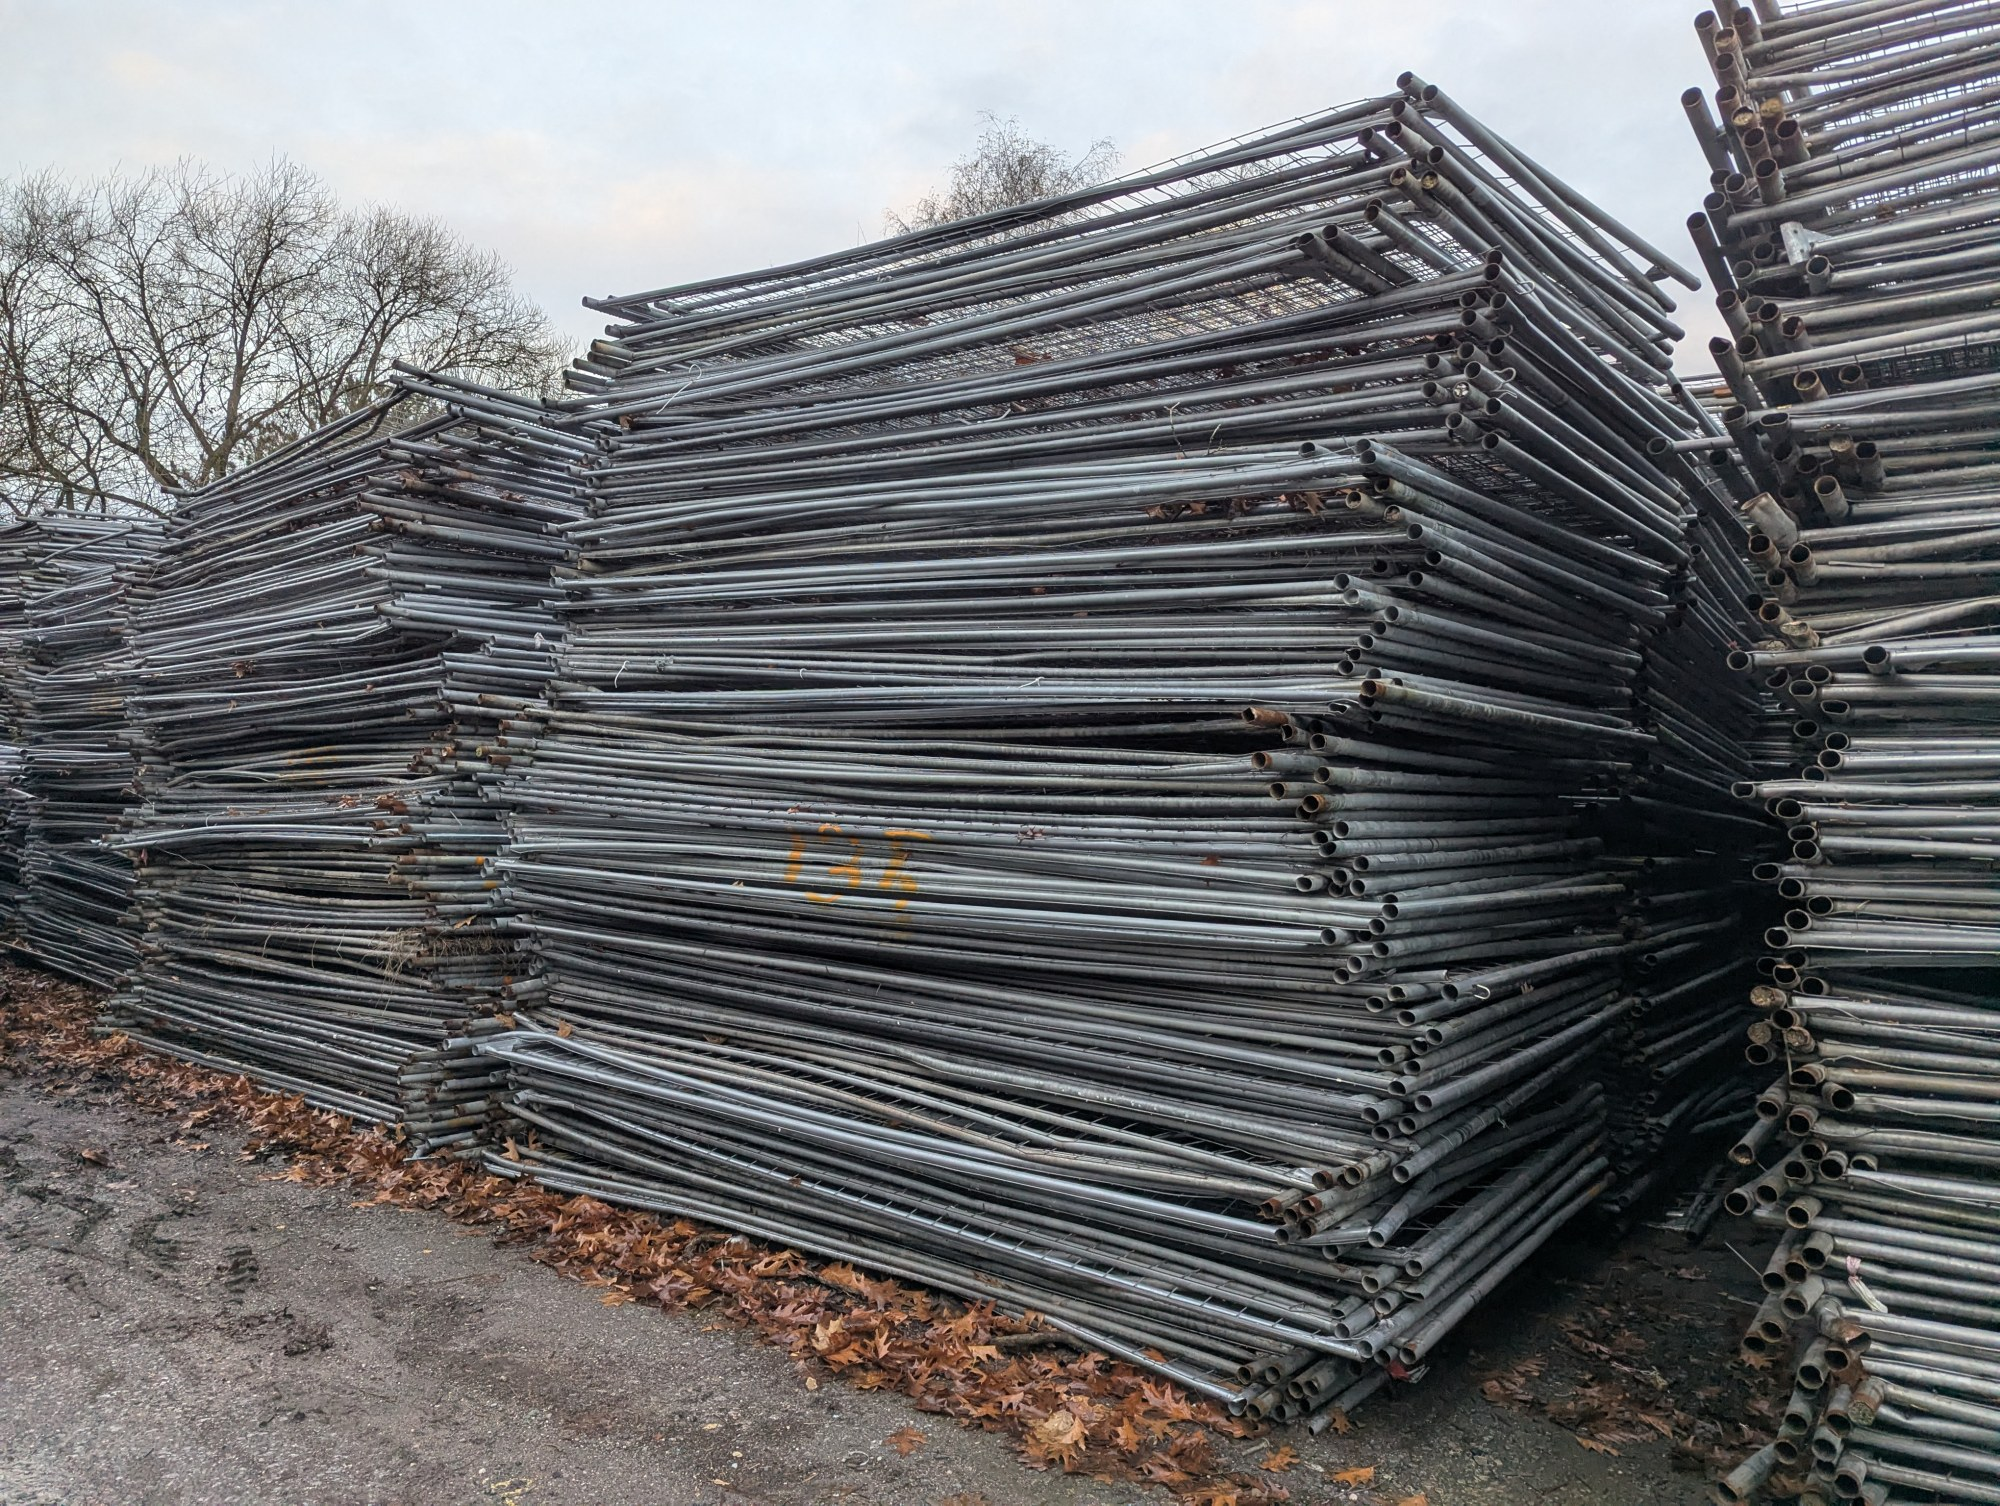
\includegraphics[width=0.92\textwidth]{abbildungen/real_stapel.jpg}
  \caption[Reale Stapelaufnahme]{Reale Aufnahme eines Stapels mobiler
  Bauzaunfelder. Zu detektieren ist die Stirnfläche der Rahmenrohre: heller
  verzinkter Kranz, dunkle Bohrung. Deutlich erkennbar sind die drei zentralen
  Schwierigkeiten -- geringe Objektgröße, hohe Objektdichte und wechselseitige
  Verdeckung durch quer liegende Rohrschäfte.}
  \label{abb:realstapel}
\end{figure}

Aus Sicht der Bildverarbeitung ist das ein unangenehmer Spezialfall: Die Objekte
sind klein (gemessen 12--36\px{} Durchmesser in den Originalaufnahmen), dicht
gepackt (im Median rund einen Objektdurchmesser Abstand zum nächsten Nachbarn),
untereinander nahezu identisch und wechselseitig verdeckt. Erschwerend kommt
hinzu, dass eine Zählaufgabe jeden einzelnen Detektionsfehler unmittelbar in das
Endergebnis überträgt: Für eine exakte Zählung von 200 Objekten wäre eine
Trefferquote von über 99,5\,\% erforderlich -- eine deutlich härtere Anforderung
als in typischen Detektionsanwendungen, in denen einzelne Fehldetektionen
tolerierbar sind.

Der eigentliche Engpass ist jedoch die Datenlage. COCO-vortrainierte Gewichte
enthalten keine Klasse \enquote{Bauzaunprofil}; das Modell muss auf einem eigens
annotierten Datensatz feinabgestimmt werden. Die Handannotation von 50--100
kleinen Boxen pro Bild über hunderte Bilder ist bei einer Abschlussarbeit nicht
leistbar. Zur Verfügung stehen lediglich neun aus Realbildern ausgeschnittene
Rohrprofile, sieben Hintergrundaufnahmen und zwei vollständig annotierte
Realbilder.

\section{Zielsetzung und Beitrag}

Der hier verfolgte Ansatz macht aus dieser Not das methodische Zentrum der
Arbeit: Trainiert wird \emph{ausschließlich} auf synthetischen Bildern, die aus
den neun Objektausschnitten und den sieben Hintergründen erzeugt werden.
Validierung und Test erfolgen auf den echten Aufnahmen. Damit ist die
Augmentierungs\-pipeline nicht mehr eine Menge von Zusatztransformationen auf einem
vorhandenen Datensatz, sondern sie \emph{ist} der Datensatz: Sie definiert die
gesamte Trainingsverteilung, und jede ihrer Entscheidungen wirkt direkt auf das
Ergebnis.

Die Arbeit verfolgt daher drei Ziele:

\begin{enumerate}
  \item \textbf{Theoretische Einordnung der Datenaugmentierung.} Was leistet
  Augmentierung formal, welche Verfahrensklassen gibt es, welche
  Besonderheiten gelten bei der Objektdetektion, und wo liegen die Grenzen?
  Kapitel~\ref{kap:augtheorie} behandelt dies unabhängig vom konkreten
  Anwendungsfall.
  \item \textbf{Vollständige Dokumentation und Begründung der konkreten
  Pipeline.} Für jede der 25 Transformationen werden Parameterbereich,
  gemessener Ist-Anteil im erzeugten Datensatz und Begründung angegeben
  (Kapitel~\ref{kap:pipeline} und \ref{kap:trainingszeit}). Die Begründung
  stützt sich dabei auf genau drei zulässige Quellen: eine Messung an den
  Realdaten, eine physikalische Randbedingung des Aufnahmegegenstands oder ein
  in der Literatur belegtes Argument. Wo keine dieser Quellen vorliegt, wird
  der Wert ausdrücklich als Annahme gekennzeichnet.
  \item \textbf{Experimentelle Bewertung.} Kapitel~\ref{kap:auswertung} misst,
  was die Pipeline auf echten Daten leistet, quantifiziert den
  Sim-to-Real-Abstand und prüft in einer kontrollierten Ablation, ob die
  aufwendigste Einzelentscheidung -- die Erzeugung physikalisch plausibler
  Verdeckung -- ihren Aufwand rechtfertigt.
\end{enumerate}

Der inhaltliche Beitrag liegt weniger in einer neuen Methode als in der
Konsequenz, mit der die Begründungspflicht durchgehalten wird. Copy-Paste-Synthese
ist ein etabliertes Verfahren \parencite{dwibedi2017,dvornik2018,ghiasi2021}; die
Frage, welche ihrer Bestandteile in einem konkreten industriellen Anwendungsfall
tragen und welche nicht, wird in der Literatur dagegen selten so kleinteilig
beantwortet, wie es hier versucht wird.

\section{Aufbau der Arbeit}

Kapitel~\ref{kap:theorie} stellt die theoretischen Grundlagen von Convolutional
Neural Networks und der YOLO26-Architektur bereit und leitet daraus die
Eignung des Verfahrens für die vorliegende Aufgabe ab.
Kapitel~\ref{kap:augtheorie} behandelt die Datenaugmentierung allgemein.
Kapitel~\ref{kap:daten} sichtet und vermisst das verfügbare Quellmaterial --
diese Messungen sind die Belegbasis für alle folgenden Parameterentscheidungen.
Kapitel~\ref{kap:pipeline} beschreibt die Synthese-Pipeline,
Kapitel~\ref{kap:trainingszeit} die davon abgegrenzte Augmentierung zur
Trainingszeit. Kapitel~\ref{kap:auswertung} wertet die Ergebnisse aus,
Kapitel~\ref{kap:diskussion} diskutiert Tragfähigkeit und Grenzen.

\begin{table}[htbp]
\centering
\caption[Verarbeitungskette]{Die Verarbeitungskette der Arbeit. Die Stufen 1--3
erzeugen die Trainingsdaten und sind Gegenstand von
Kapitel~\ref{kap:pipeline}.}
\label{tab:kette}
\small
\begin{tabularx}{\textwidth}{@{}llX@{}}
\toprule
\textbf{Stufe} & \textbf{Skript} & \textbf{Aufgabe} \\
\midrule
0 & \code{analyze\_data.py} & Sichtung und Vermessung des Quellmaterials; erzeugt
alle Messwerte, auf die sich die Parameterbegründungen berufen \\
1 & \code{matting.py} & Freistellen der neun Objektausschnitte, weiche Alphamasken \\
2 & \code{occluders.py} & Extraktion echter Rohrschäfte als Okkluder-Bibliothek \\
3 & \code{generate.py} & Bildsynthese mit exakter Sichtbarkeitsrechnung \\
4 & \code{train.py} & Training, Parametertabelle mit Begründungen \\
5 & \code{evaluate.py} & eigenständiges Bewertungsframework (COCO-Metriken, Zählfehler) \\
6 & \code{experiment.py} & Inferenzparameter-Sweeps, Okklusionsablation, Modellvergleich \\
7 & \code{report.py} & Diagramme und Ergebnistabellen \\
\bottomrule
\end{tabularx}
\end{table}
